\let\negmedspace\undefined
\let\negthickspace\undefined
\documentclass{beamer}
\usetheme{CambridgeUS}
\usepackage{csquotes}
\usepackage{comment}
\usepackage{enumerate}
\usepackage{amsmath,amssymb,amsthm}
\usepackage{graphicx}
\let\vec\mathbf
\newcommand{\myvec}[1]{\ensuremath{\begin{pmatrix}#1\end{pmatrix}}}
\providecommand{\brak}[1]{\ensuremath{\left(#1\right)}}
\providecommand{\pr}[1]{\ensuremath{\Pr\left(#1\right)}}


     \title{Assignment 1}
     \author{AKKASANI YAGNESH REDDY \\
     CS21BTECH11003 \\
     ICSE 2019 11c }
     \date{\today}
\logo{\large \LaTeX{}}
     
     \begin{document}
     \begin{frame}
     \maketitle    
     \end{frame}
     
     \logo{}
     
     \begin{frame}{Outline}
    \tableofcontents
     \end{frame}

   \section{Question}
   \begin{frame}{Question}
   \begin{block}{Question}
           In the given figure, $ABCDE$ is a pentagon inscribed in a circle such that $AC$ is a diameter and side $BC//AE$. If $ \angle{BAC} = 50^{\circ} $, find giving reasons:
    \begin{enumerate}
    \item $\angle ACB$
    \item $\angle EDC$
    \item $\angle BDC$
    \end{enumerate}
Hence prove that $BE$ is also a diametre.
       \end{block}
     \end{frame}
      \section{figure}
     \begin{frame}{figure}
       \begin{figure}[h!]  
        % \graphicspath{{./Figures/}}  
            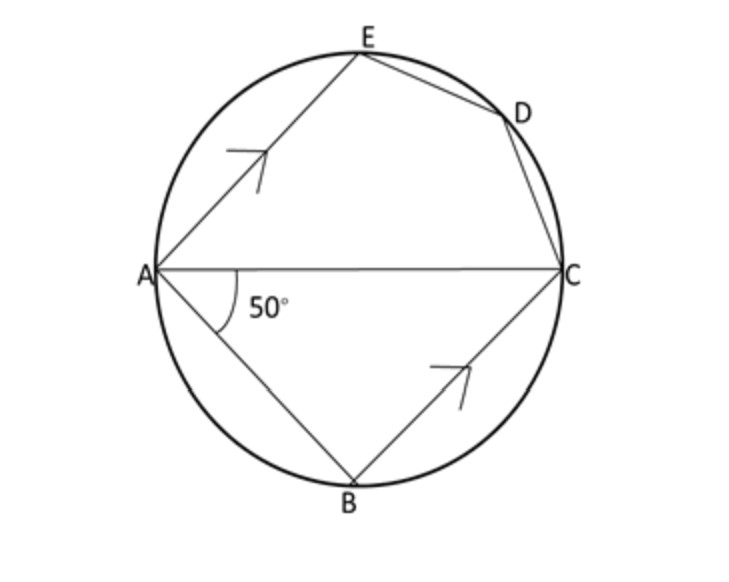
\includegraphics[]{question}
            \label{Fig1} 
             \caption{}
      \end{figure}
         
     \end{frame}
     
     \section{solution}
     \begin{frame}{Solution}
       \begin{enumerate}
    \item $\triangle ABC $,  $ \angle ABC = 90^{\circ} $ (angle in a semicircle)
    \begin{align}
      \angle{CBA} +\angle BCA+\angle CAB &=180^{\circ}\\
        90^{\circ}+\angle BCA+50^{\circ} &=180^{\circ}\\
        \angle BCA &=40^{\circ}
    \end{align}
    \end{enumerate}
     \end{frame}
     
     \begin{frame}{Solution}
     \begin{enumerate}
     \setcounter{enumi}{1}
          \item $AE \backslash\backslash BC$
    \begin{align}
     \angle CAE=\angle ACB=40^{\circ}(pair of alternate angles)
     \end{align}
     In cyclic quadrilateral $ACDE$
     \begin{align}
         \angle CAE + \angle EDC=180^{\circ}
     \end{align}
      opposite angles of a cyclic quadrilateral add upto $180^{\circ}$ \\
      \begin{align}
        40^{\circ}+\angle EDC=180^{\circ}\\
        \angle EDC =140^{\circ}
      \end{align}
            \end{enumerate}
            \end{frame}
            
        \begin{frame}{solution}
        
        
        \begin{enumerate}
            \setcounter{enumi}{2}
        
        \item $\angle BEC= \angle BAC=50^{\circ}$(angles in the same segment)
      \item For the proof of diameter
      \end{enumerate}
      \begin{align}
      \angle AEB=90^{\circ}-50^{\circ}=50^{\circ}\\
      \angle EBC=40^{\circ}\\
      \angle ECB=90^{\circ}
            \end{align}
$\therefore$ BE is a diameter
        \end{frame}
        
       \section{steps for python plot}
       \begin{frame}{steps for python plot}
       \begin{enumerate}
    \item Let $\vec{O}$ be the origin \\ 
              \begin{align}
               \vec{O}=\myvec{0\\0}
               \end{align}
               Draw a circle with centre at $\vec{O}$ and radius $r=1$\\
  Without losing generality lets assume $AC$ to be along $x-axis$.This gives points $\vec{A}$ and $\vec{C}$.
  \begin{align}
      \vec{A}&=\myvec{-1\\0}\\
      \vec{C}&=\myvec{1\\0}
  \end{align}
  Plot the points A,B,O and join them.
  \end{enumerate}
       \end{frame}
       
       \begin{frame}{steps for pyhton plot}
       \begin{enumerate}
           \setcounter{enumi}{1}
             \item The angle between $OA$ and $OB$ is $80^{\circ}$.
   So, coordinates of $\vec{B}$ are \\
   \begin{align}
       \vec{B}=\myvec{-\cos(80^{\circ})\\-\sin(80^{\circ})}
   \end{align}
   Plot B.
       \end{enumerate}
       \end{frame}
        
        \begin{frame}{steps for python plot}
        \begin{enumerate}
            \setcounter{enumi}{2}
               \item The angle between $OC$ and $OE$ is $80^{\circ}$
   So,cordinates of $\vec{E}$ are
   \begin{align}
       \vec{E}=\myvec{\cos(80^{\circ})\\\sin(80^{\circ})}
   \end{align}
   
   Plot E.
        \end{enumerate}
                \end{frame}
                
        \begin{frame}{steps for python plot}
        \begin{enumerate}
            \setcounter{enumi}{3}
               \item $\vec{D}$ can be anywhere between $\vec{E}$ and $\vec{C}$
   lets plot the symmetric point then angle between $OD$ and $OC$ is $40^{\circ}$.
   \begin{align}
       \vec{D}=\myvec{\cos(40^{\circ})\\\sin(40^{\circ})}
   \end{align}
   Plot D.\\
   \item Now join $AB$ $BC$ $CD$ $DE$ $EA$ and $BE$.
        \end{enumerate}
        \end{frame}
        
        \begin{frame}{genarated figure}
         The python figure obtained from following the above steps is
  \begin{figure}[h!]  
        % \graphicspath{{./Figures/}}  
            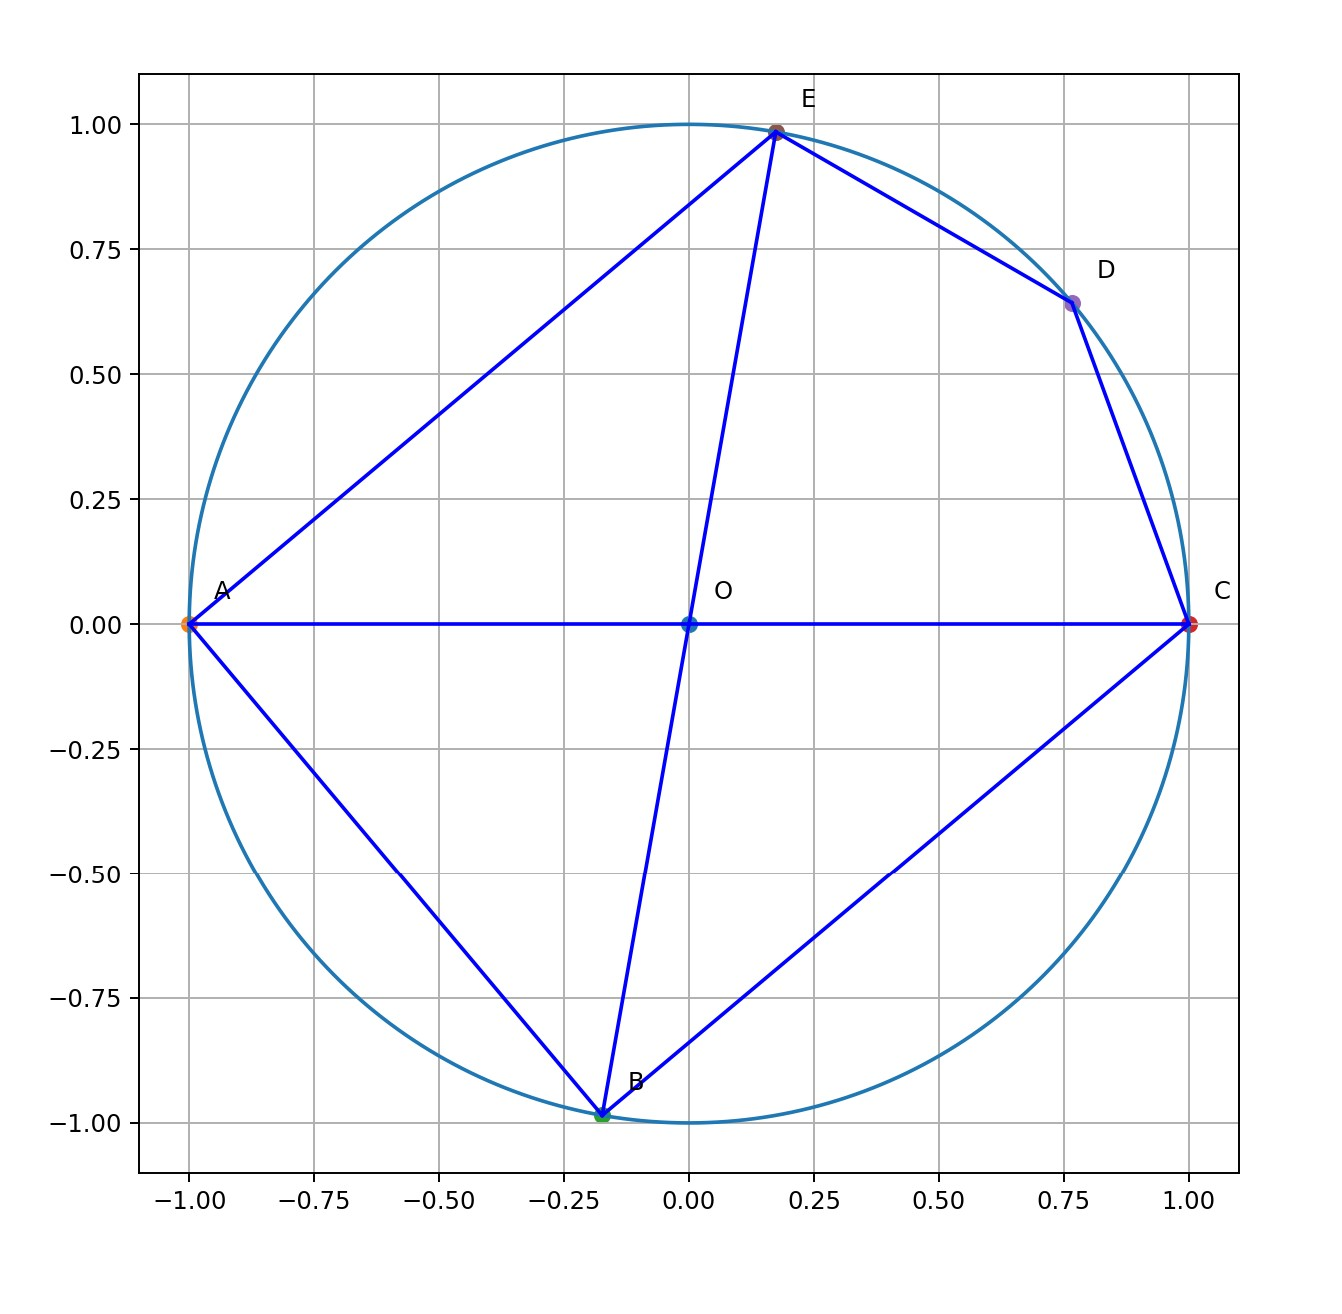
\includegraphics[scale=0.25]{pythonfig.jpg}
            \label{Fig2} 
             \caption{}
      \end{figure}
        
        \end{frame}


   \begin{frame}{Table}
   The parameters required o construct the figure in python are given in the below table .    
      
\begin{table}[h!]
    \centering
    \begin{tabular}{|c|c|c|} \hline
    \textbf{Symbol} & \textbf{Value} & \textbf{description} \\ \hline
 $r$ & $1$ &  value of r does not change our results \\ \hline
 $\theta$ & $40^{\circ}$ & $\angle EAC$,calculated \\ \hline
 $\vec{A}$ &  $\myvec{-1\\0}$  & assumed\\ \hline 
 $\vec{C}$ & $\myvec{1\\0}$ & assumed \\ \hline
 $\vec{B}$ & $\myvec{-r\cos(2\theta)\\-r\sin(2\theta)}$ & calculated \\ \hline
 $\vec{E}$ & $\myvec{r\cos(2\theta)\\r\sin(2\theta)}$ & calculated \\ \hline
 $\vec{D}$ & $\myvec{r\cos(\theta)\\r\sin(\theta)}$ & calculated \\ \hline
 \end{tabular}
   % \caption{Caption}
    \label{tab:my_label}
\end{table}
\end{frame}
\end{document}